\documentclass[12pt,fleqn]{article}\usepackage{../../common}
\begin{document}
Ders 1

Elektrik ve Manyetik Etkile�imler dersine ho�geldiniz. Ben Professor
Carlson, ben fizi�i �ok seviyorum onun i�in buraday�m. Ben teorik
fizik�iyim, her g�n matematikle u�ra��yorum yani, bu benim i�im, d�nyan�n
nas�l olmas� gerekti�ini / olabilece�ini anlamaya u�ra�mak, teorisyenler
bununla me�guld�rlar. Bir de deneyci arkada�lar�m�z var tabii, onlar
d�nyan�n ger�ekte nas�l oldu�uyla alakal�d�r. Bu iki kanat, biz ve onlar
biraraya geliriz sonra, bulu�uruz, konu�uruz. Anla�amad���m�z zaman yeni
bir �eyler ��renmemiz gerekti�ini anlar�z, b�yle devam eder.

Fizik size net dusunmeyi ogreten derslerden biridir. Cogunlukla ufak bir
mantikli prensip demeti olur elimizde, ve bu demeti mantik zinciri kura
kura bir sonraki daha buyuk anlayisa ulasmamiz mumkun olur. 

Ba�layal�m o zaman. �lk kanun Columb'un Kuvvet Kanunu.

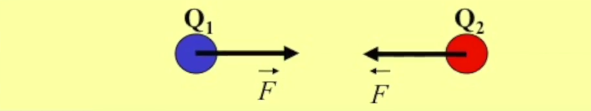
\includegraphics[width=20em]{elecmag_01.png} 























\end{document}
























